\documentclass[a4paper,12pt]{report}

\usepackage{alltt, fancyvrb, url}
\usepackage{graphicx}
\usepackage[utf8]{inputenc}
\usepackage{hyperref}
\usepackage{float}
\usepackage{textcmds}
\usepackage{a4wide}

\usepackage[italian]{babel}

\usepackage[italian]{cleveref}

\title{
\textbf{AirLine Traffic Simulator}
\\Relazione di progetto
\\Programmazione ad Oggetti
}
\date{Agosto 2021}

\author{
Severi Andrea
\\Foschi Andrea
\\Rodilosso Daniel
}

\begin{document}

\maketitle

\tableofcontents

\chapter{Analisi}
Il gruppo si pone come obiettivo quello di realizzare un videogioco sulla gestione del traffico aereo, ispirandosi al gioco mobile \href{https://youtu.be/KTH084KeFBc}{\underline{“Flight Control”}}.
\\
L’obiettivo del giocatore sarà quello di far atterrare il maggior numero di aerei che compariranno progressivamente sulla mappa, evitando di farli collidere tra di loro (causando la fine del gioco).
\\
Il giocatore gestirà personalmente la direzione di ogni velivolo, disegnandone il percorso che dovrà seguire ciascun aereo, con il mouse.
\\
La difficoltà di gioco aumenterà con l’aumentare del numero di aerei che saranno fatti atterrare.

\section{Requisiti}

\paragraph{Funzionalità necessarie:}

\begin{itemize}
    \item Disegnare correttamente con il mouse il percorso che l’utente vuol far seguire al velivolo selezionato.
    
    \item Implementare un’intelligenza artificiale, che muoverà gli aerei quando non avranno una destinazione scelta dall’utente (l’aereo una volta entrato nella mappa non potrà uscire, ma dovrà continuare a volare all’interno di essa).
    
    \item Realizzare una gestione efficiente degli aerei in entrata sulla mappa e il relativo atterraggio quando raggiungeranno la pista di atterraggio.
    
    \item Salvataggio degli score dei vari utenti in un file apposito, che verrà reso disponibile ad ogni avvio.
    
    \item Gestione della difficoltà crescente durante la partita.
\end{itemize}

\paragraph{Funzionalità opzionali:}
\begin{itemize}
    \item Creazione e aggiunta di mappe dinamiche (es: implementazione di oggetti che causeranno la distruzione dell’aereo se sorvolati, animazioni dinamiche nella mappa).
    
    \item Implementazione suoni di gioco.
    
    \item Aerei speciali, con velocità diverse.
    
    \item Gestione del vento: questo causerà una maggiore o minore velocità degli aerei durante la partita.
\end{itemize}

\paragraph{\textbf{Challenge principali:}}
\begin{itemize}
    \item “Fluidità" delle animazioni (tracciamento della rotta, movimento degli aerei, atterraggio degli aerei, collisione tra gli aerei).
    
    \item Corretta implementazione del pattern MVC.
    \item Gestione della difficoltà (crescente durante la partita).
\end{itemize}

\section{Analisi e modello del dominio}
AirLine Traffic Simulator dovrà essere in grado di gestire lo spawn (Spawn) degli aerei (Plane) e la loro entrata in partita dopo un quantitativo di tempo prefissato. 
\\
È presente una \textbf{Mappa di gioco} (Seaside) a tema aeroporto.
\\	
All’inizio della \textbf{Partita} (Game) verranno creati e appariranno in maniera sequenziale gli \textbf{Aerei} sulla mappa, che seguiranno un \textbf{percorso casuale} (gli Aerei ancora non possiedono una rotta specifica da seguire ma semplicemente si muovono nella Mappa). 
\\
In questo caso quando un aereo non possiede una rotta specifica dovrà muovervi verso una direzione indicata dall’\textbf{algoritmo di I.A.}
\\
Compito dell’utente è quello di far atterrare gli Aerei sulle \textbf{Piste di Atterraggio} (AirStrip) presenti sulla mappa.
\\
Gli Aerei presenti nel gioco potranno essere di più tipologie (PlaneType), aventi velocità diverse.
\\
Un Aereo potrà atterrare quando sarà in prossimità dell’area di atterraggio, resa disponibile dalla Pista stessa.
\\
Sarà quest’ultima (AirStrip) a convalidare la possibilità o meno di fare atterrare il velivolo in caso di contatto con l'area di atterraggio.
\\
Per ogni Aereo che riuscirà ad atterrare correttamente, il Giocatore (User) incrementerà il proprio \textbf{Punteggio} con un valore deciso a priori.
\\
Il \textbf{Giocatore} potrà eseguire le seguenti operazioni sull’Aereo che vuole muovere:
\begin{itemize}
    \item selezionare l’Aereo che vuole controllare.
	\item disegnare il percorso (Path) che poi l'Aereo dovrà correttamente seguire.
\end{itemize}

\noindent È stato pensato di implementare degli indicatori all’interno dell'area di gioco per segnalare gli aerei in arrivo da fuori dalla Mappa.
\\
Questi segnali scompariranno non appena l’aereo entrerà in partita.

\paragraph{Il giocatore \underline{perde} se:}
\begin{itemize}
    \item fa collidere gli aerei tra di loro in volo
    \item urta il bordo con un aereo presente in partita
\end{itemize}
In entrambi in casi, viene generata un'esplosione a video.
\\
Nel tentativo di evitare ciò, allo scorrere del \textbf{Tempo di gioco}, altri aerei che dovranno essere fatti atterrare, compariranno sulla Mappa, con maggiore frequenza in base al punteggio.
\\
É possibile mettere anche in \textbf{pausa} la partita tramite pulsante dall’interfaccia di gioco.
\\
Alla fine della Partita, il Giocatore avrà ottenuto un punteggio finale, che sarà salvato su \textbf{file}. Se sarà sufficiente per entrare in \textbf{Classifica}, verrà inserito in quest’ultima.
\\
Dal \textbf{Menù Principale}, oltre che iniziare una nuova partita, si potrà visualizzare tale classifica.


% da tenere per dopo
% La classifica prevederà un File (di estensione “.json”) che manterrà in memoria i punteggi dei giocatori una volta terminata l’applicazione.

\chapter{Design}
\section{Architettura}
L’architettura di Airline Traffic Simulator segue l’architettura M.V.C. \newline
Abbiamo deciso di utilizzare il design classico di questo pattern.
\\
Utilizzando la libreria di JavaFX abbiamo un unione molto dipendente tra la parte di View e quella di Controller.
Questo perché la View stessa viene disegnata e implementata tramite un file .fxml, il cui scheletro deve essere presente all’interno del Controller.
Ciò genera da una parte un ottimizzazione per la realizzazione dei due componenti, dall’altra però va inevitabilmente a creare un forte legame di dipendenza.
In fatti nel caso in cui successivamente si volesse cambiare libreria grafica sostituendo JavaFx, la parte di Controller, andrebbe interamente riscritta, rendendo meno semplice la sostituzione in blocco della View stessa.
\\
AltSim implementa Seaside ed è il Controller centrale del sistema, ad esso sono infatti collegati i vari Controller degli oggetti chiave dell’applicazione (Plane, Map, Airstrip ***). 
All’interno di Seaside l’utente sarà in grado di disegnare e controllare la rotta dei vari Plane che entreranno in partita.
Una particolare attenzione merita il GameEngine.
Esso si occuperà di monitorare i vari oggetti durante la partita (come ad esempio per il caso di Plane, verificare se collide con un altro Plane, o essendo in prossimità della AirStrip far atterrare il Plane stesso) e intraprendere le azioni di aggiornamento e notifica adeguati. Abbiamo riscontrato che un vantaggio di utilizzare questa architettura è che è possibile inserire altre Entità o modifiche all’interno del nostro gioco senza impattare la complessità di progettazione.

\clearpage

\section{Design dettagliato}
\subsection{Severi Andrea}
Durante le fasi di analisi, è emersa l'esigenza di mantenere i dati relativi alle partite degli utenti in un file apposito e di estrapolarne una classifica contenente i migliori giocatori. Per cui, uno dei miei principali obiettivi era l'apportare un contributo per la creazione dell'utente e del salvataggio del suo punteggio.
\subsubsection{User}
Occupandomi personalmente dell'interfaccia grafica dell'applicazione, avevo subito in mente ogni singolo passo per la realizzazione dello \texttt{User}. 
Le sue caratteristiche sono l'univocità del nome utente da scegliere nel menù principale e il punteggio, attribuito successivamente in partita. Nonostante la scelta di soltanto due parametri, a mio vedere sufficienti per lo stato attuale dell'applicazione, ho deciso di utilizzare il pattern \textbf{Builder} per la creazione dell'utente. La motivazione è la predilezione per un pattern che fornisce chiarezza nella lettura del codice, rispetto a un costruttore, e per fornire una base solida di partenza nel caso di futura aggiunta di nuove caratteristiche da attribuire all'utente stesso.

\begin{figure}[H]
    \begin{center}
        \centering
        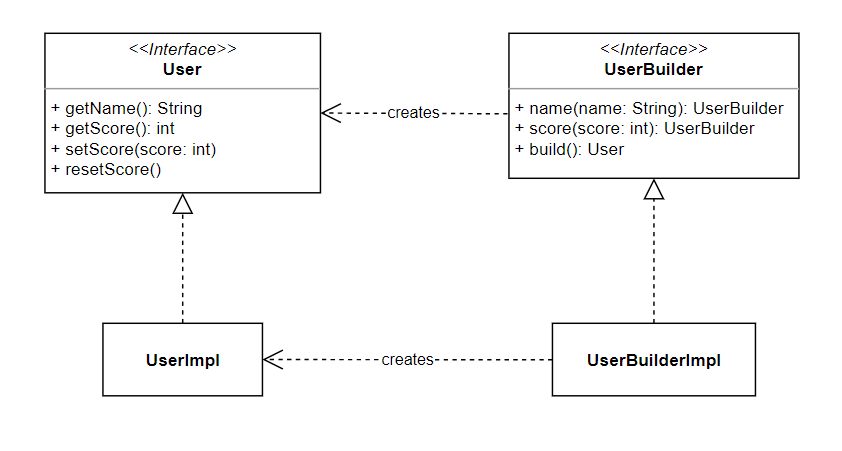
\includegraphics[width=\textwidth]{img/Severi/User.png}
    \end{center}
    \caption{Creazione di \texttt{User}}
    \label{img:user}
\end{figure}

\subsubsection{UserRecords}
Al fine di mantenere in memoria la creazione degli utenti e dell'attribuzione loro di un punteggio, è stato necessario creare una classe che potesse gestire la realizzazione di una \textit{hidden directory} all' avvio dell'applicazione con al suo interno il file dei punteggi. Inizialmente, l'approccio scelto è stato la realizzazione della classe \texttt{RecordsValidation}, la quale controllava sia dell'esistenza di directory e file sia della creazione di essi. Tale metodo non era di mio gradimento, per cui ho deciso di separare le due parti di logica utilizzando il pattern \textbf{Adapter}, in modo tale da poter riutilizzare i metodi necessari anche per \texttt{UserRecordsImpl}, evitando ripetizioni di codice e violazioni del principio DRY. Per quanto riguarda l'interfaccia \texttt{UserRecords} ho optato per il pattern \textbf{Strategy}, in quanto contiene algoritmi utilizzabili per qualsiasi tipo di file si voglia usare. In prima battuta, la scelta è ricaduta su due estensioni: \textit{.csv} e \textit{.json}. La decisione di usare \textit{.json} è stata dettata dal fatto che è più facilmente manipolabile, grazie alla libreria \href{https://github.com/google/gson}{\underline{Gson}}, rispetto alla controparte, di cui è possibile trovare librerie di terze parti, ma che sono meno convincenti, data la scarsa accuratezza nell'attribuzione ai nomi dei metodi e il minor sviluppo da parte del team di creazione\footnote{In particolare si fa riferimento alla libreria \href{https://github.com/jtablesaw/tablesaw}{\underline{Tablesaw}}}. Per cui \texttt{UserRecordsImpl} contiene l'implementazione json degli algoritmi di inserimento, attribuzione del punteggio e controllo riguardo la presenza dell'utente nel file.
\begin{figure}[H]
    \begin{center}
        \centering
        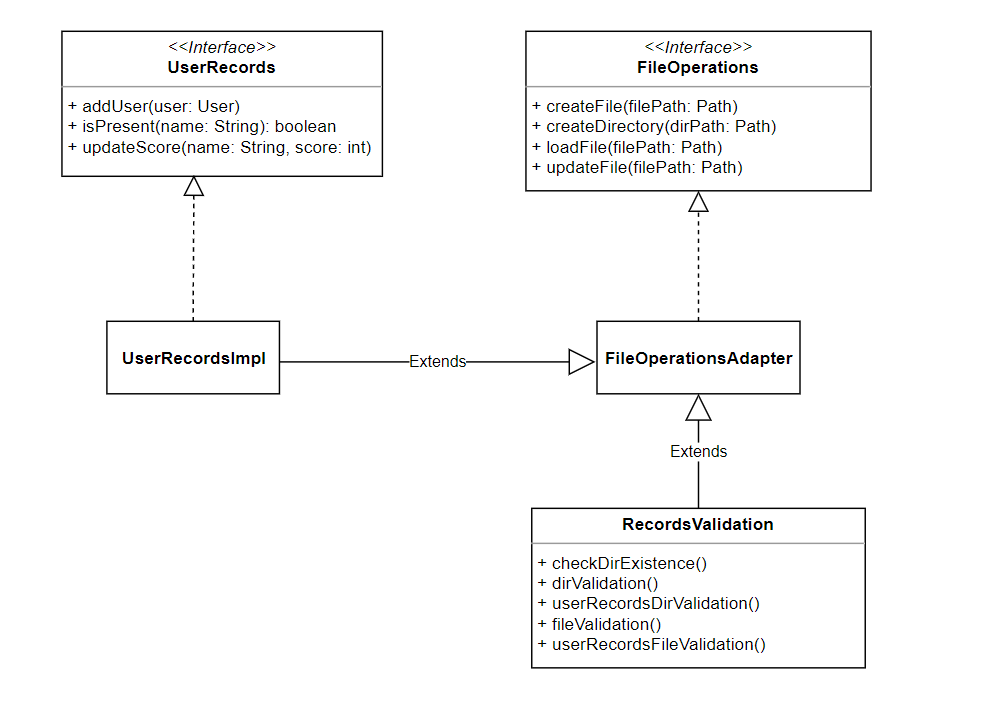
\includegraphics[width=\textwidth]{img/Severi/Records.png}
    \end{center}
    \caption{Gestione del file}
    \label{img:records}
\end{figure}
\subsubsection{Leaderboard}
Per quanto riguarda la realizzazione della classifica ho pensato a un semplice algoritmo di comparazione fra gli utenti, basato ovviamente sul punteggio, volto all'utilizzo degli \textit{Stream}, introduzione nella versione 8 di Java, nonchè uno dei pilastri del corso. 
\begin{figure}[H]
    \begin{center}
        \centering
        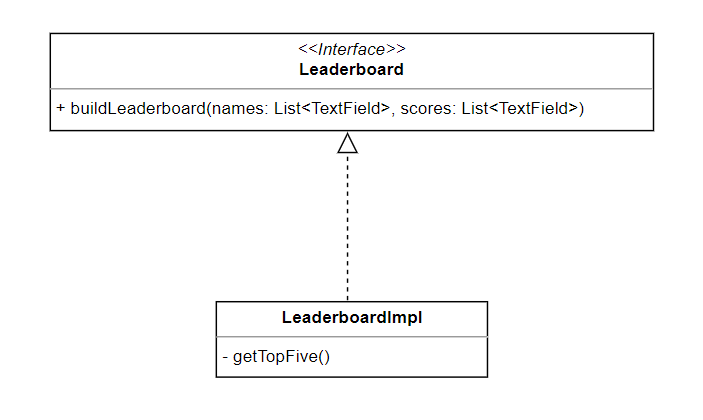
\includegraphics[width=\textwidth]{img/Severi/Leaderboard.png}
    \end{center}
    \caption{Gestione della classifica}
    \label{img:leaderboard}
\end{figure}

\subsubsection{NameQuality}
La classe \texttt{NameQuality} consente di controllare il nome inserito dall'utente nel menù principale e di valutarne la qualità, facendo affidamento all'enum \texttt{NameResult}. Al fine di ottenere nomi semplici e di lunghezza finita, ho deciso di implementare un pattern regex, il quale restringe la scelta del nome a un lunghezza massima di 12 lettere e l'utilizzo di soli numeri e lettere. In tal modo, l'input viene verificato tramite espressione regolare e viene ottenuto uno dei seguenti valori:
\begin{itemize}
    \item \qq{\texttt{CORRECT}}: il nome segue i canoni imposti
    \item \qq{\texttt{EMPTY}}: il nome è vuoto o contiene soli spazi
    \item \qq{\texttt{TOO\_LONG}}: il nome è più lungo di 12 caratteri
    \item \qq{\texttt{WRONG}}: il nome contiene caratteri non validi
    \item \qq{\texttt{TAKEN}}: il nome è già in uso
\end{itemize}
\noindent In base al valore ottenuto, successivamente si agisce in maniera diversa in interfaccia grafica. Tale scelta mi ha permesso di utilizzare spesso l'\texttt{Enum} nella View per inviare informazioni all'utente riguardo il nome selezionato.

\begin{figure}[H]
    \begin{center}
        \centering
        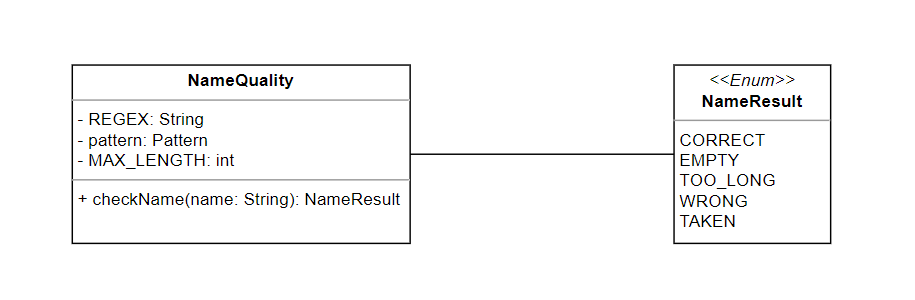
\includegraphics[width=\textwidth]{img/Severi/Name.png}
    \end{center}
    \caption{Controllo sul nome}
    \label{img:name}
\end{figure}

\subsection{Foschi Andrea}
\subsubsection{Piste di atterraggio}
Mi sono personalmente occupato di una delle due componenti fondamentali del gioco: le piste di atterraggio. Tale componente si suddivide in due macrocategorie: quelle che gestiscono l’atterraggio degli aerei standard, e quelle che gestiscono l’atterraggio degli elicotteri (in realtà per quest’ultima categoria vi è nel codice una sola predisposizione a tale tipo di velivolo per implementazioni future, a causa della mancata implementazione degli elicotteri).
\begin{figure}[H]
    \begin{center}
        \centering
        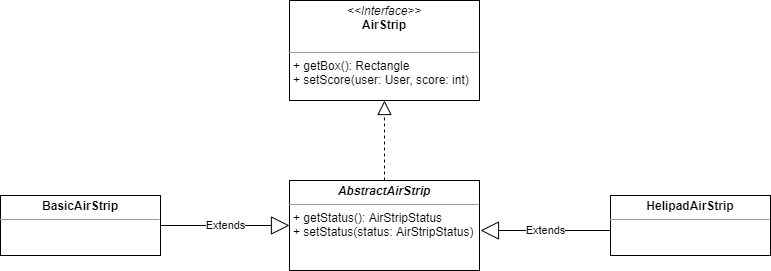
\includegraphics[width=\textwidth]{img/Foschi/Airstrip.png}
    \end{center}
    \caption{Pista di atterraggio}
    \label{img:airstrip}
\end{figure}

\subsubsection{Atterraggio degli aerei e verifica delle collisioni}
Per fare in modo che la pista di atterraggio prenda in ingresso un aereo da far atterrare è stato necessario definire un controller del sistema. In questo modo la pista di atterraggio, tramite il metodo intersects() fornito da JavaFX, può accertare la collisione avvenuta e notificare l’evento alle altre componenti dell’applicazione. Si denota l’utilizzo dell’Enum AirStripStatus, che può assumere i seguenti valori:
\begin{itemize}
    \item \qq{\texttt{FREE}}: la pista è in grado di ricevere un aereo da far atterrare;
    \item \qq{\texttt{BUSY}}: la pista sta facendo atterrare un aereo e non è in grado di riceverne altri;
    \item \qq{\texttt{DISABLED}}: la pista è momentaneamente non disponibile.
\end{itemize}
\begin{figure}[H]
    \begin{center}
        \centering
        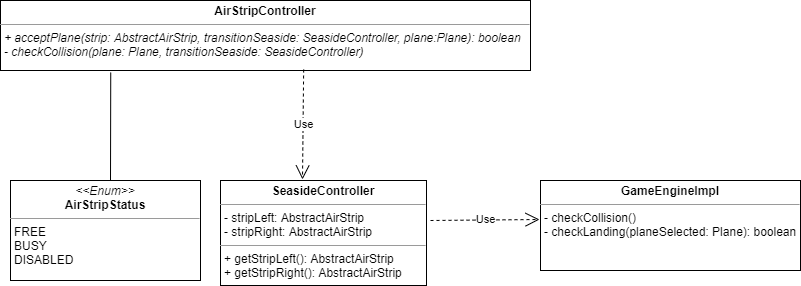
\includegraphics[width=\textwidth]{img/Foschi/AirStripController.png}
    \end{center}
    \label{img:airstrip-controller}
\end{figure}

\clearpage

\subsection{Rodilosso Daniel}

\chapter{Sviluppo}
\section{Testing automatizzato}
\subsection{Severi Andrea}
\subsection{Foschi Andrea}
\subsection{Rodilosso Daniel}

\section{Metodologia di lavoro}
\subsection{Severi Andrea}
\subsection{Foschi Andrea}
\subsection{Rodilosso Daniel}

\section{Note di sviluppo}
\subsection{Severi Andrea}
\subsection{Foschi Andrea}
\subsection{Rodilosso Daniel}

\chapter{Commenti finali}
\section{Autovalutazione e lavori futuri}
\subsection{Severi Andrea}
Questo progetto mi ha sicuramente aiutato a crescere come sviluppatore e mi ha fatto appassionare maggiormente a un linguaggio che inizialmente reputavo difficile e temibile, tanto dall'aver acquistato volumi quali \href{https://www.amazon.it/Effective-Java-Joshua-Bloch/dp/0134685997}{\qq{\underline{\textit{Effective Java}}}} e \href{https://it.wikipedia.org/wiki/Design_Patterns}{\qq{\underline{\textit{Design Patterns}}}}. Sono consapevole del fatto che ho ancora molto da migliorare, ma cerco sempre di documentarmi al meglio per trovare tecniche e approcci migliori alla scrittura del codice. Ho sempre cercato di rispettare regole (lingua inglese, stile) e convenzioni, affinchè il codice sia leggibile e comprensibile da tutti. Per il futuro voglio sicuramente concentrarmi su uno studio più approfondito dei Design Patterns e su una scrittura più professionale del codice, magari creando nuovi progetti da zero o andando a rimodellare quello appena creato. Inoltre conoscere sempre di più la programmazione ad oggetti che tanto mi ha appassionato, con lo studio possibilmente anche di altri linguaggi.

\subsection{Foschi Andrea}
\subsection{Rodilosso Daniel}

\clearpage

\section{Difficoltà incontrate e commenti per i docenti}
\subsection{Severi Andrea}
Come gruppo, nonostante la comunicazione costante, è sicuramente mancata un po' sintonia, conoscendosi poco e sarebbe servita una migliore organizzazione, in modo tale da non riscrivere parti già fatte e concentrarsi sulle singole parti. Forse poteva servire per evitare di fallire la deadline precedente. 
Il corso mi ha aiutato a ragionare molto di più sul problema da risolvere, piuttosto che buttarsi subito sulla scrittura di codice. Nonostante sia un corso difficile, ho apportato il massimo impegno e penso ciò verrà ripagato.
Una cosa che non mi è piaciuta a pieno è stata la spiegazione su JavaFX, poichè non ero bene a conoscenza di ciò che realmente offre e che pensavo si dovesse implementare da zero. Nonostante questo, corso fatto molto bene.

\subsection{Foschi Andrea}
\subsection{Rodilosso Daniel}

\appendix
\chapter{Guida utente}
\section*{Home Page}
All'avvio dell'applicazione, sono presenti 4 pulsanti: \texttt{START, LEADERBOARD, CREDITS, EXIT}, per avviare una nuova partita, visualizzare la classifica dei migliori giocatori, visionare i riconoscimenti per ognuno dei membri del gruppo e uscire dall'applicazione.
\begin{figure}[H]
    \begin{center}
        \centering
        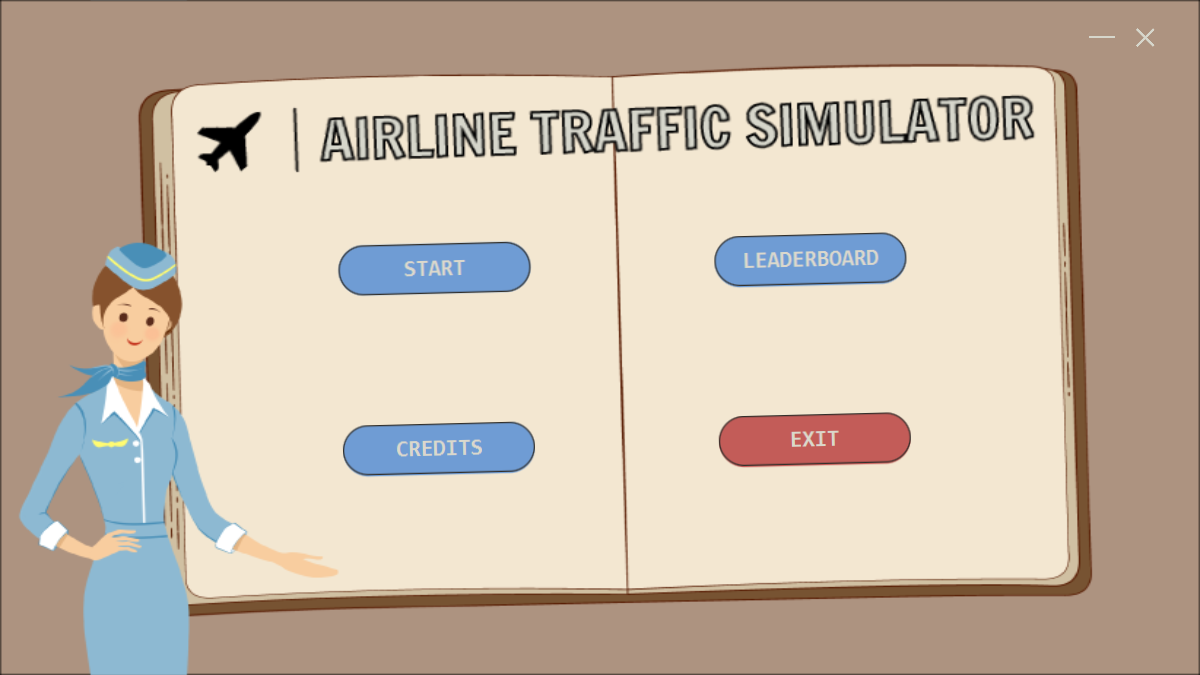
\includegraphics[width=\textwidth]{img/GuidaUtente/Home.png}
    \end{center}
    \caption{Home Page}
    \label{img:homepage}
\end{figure}

\section*{MapChoice}
Tramite questa schermata è possibile scegliere una delle mappe disponibili, al momento solo una delle quattro. Inoltre è obbligatorio scegliere un nome, come suggerisce l'info per iniziare una nuova partita.
\begin{figure}[H]
    \begin{center}
        \centering
        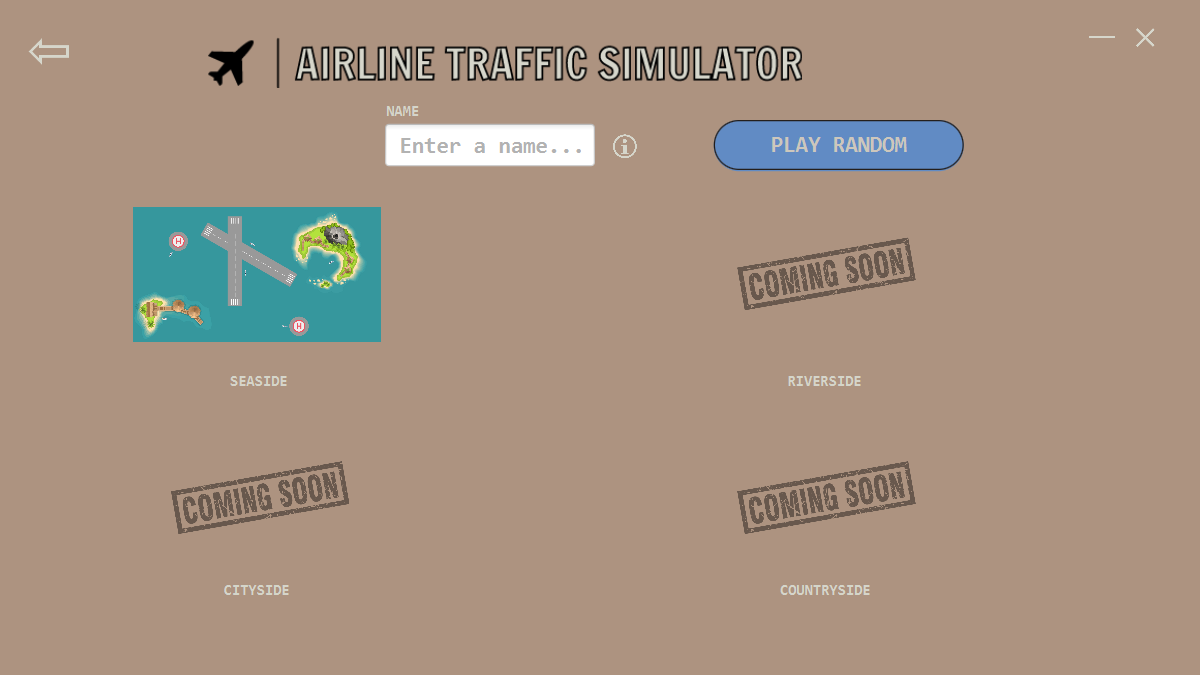
\includegraphics[width=\textwidth]{img/GuidaUtente/MapChoice.png}
    \end{center}
    \caption{Scelta della mappa}
    \label{img:mapchoice}
\end{figure}

\clearpage

\section*{Classifica}
In questa schermata è possibile vedere la top 5 dei migliori giocatori di AirLine Traffic Simulator con relativo nome e punteggio.
\begin{figure}[H]
    \begin{center}
        \centering
        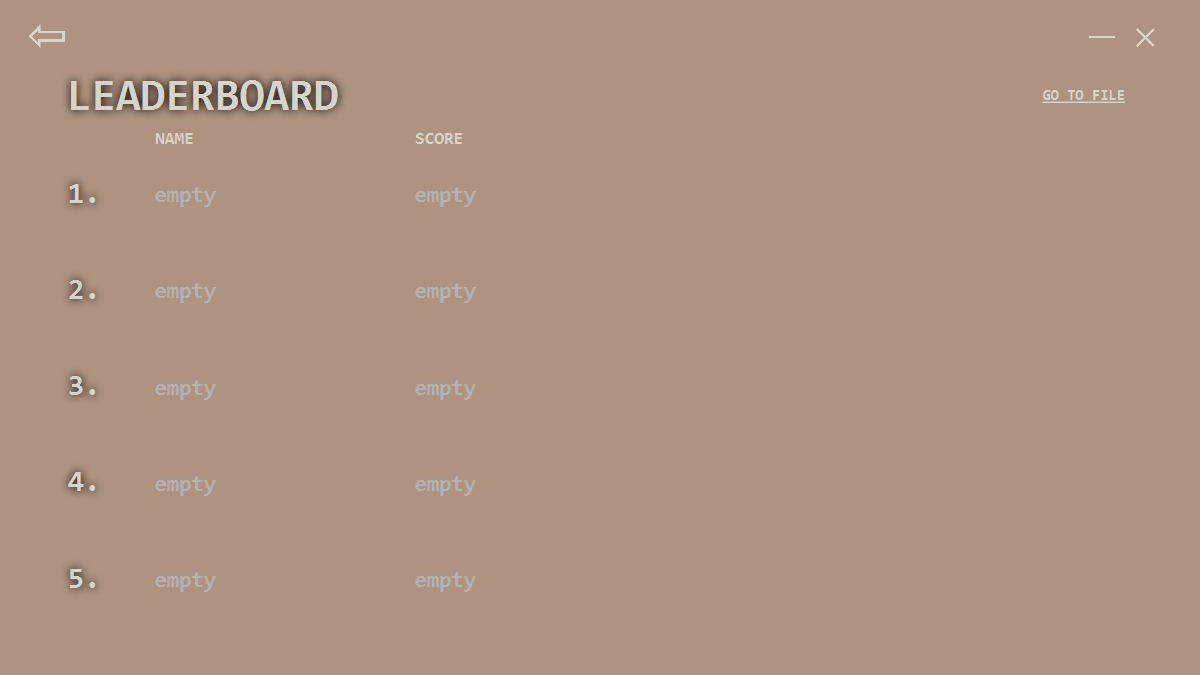
\includegraphics[width=\textwidth]{img/GuidaUtente/Leaderboard.png}
    \end{center}
    \caption{Classifica}
    \label{img:leaderboard-png}
\end{figure}

\clearpage

\section*{Credits}
Schermata per una veloce visione del lavoro svolto dai singoli partecipanti al gruppo.
\begin{figure}[H]
    \begin{center}
        \centering
        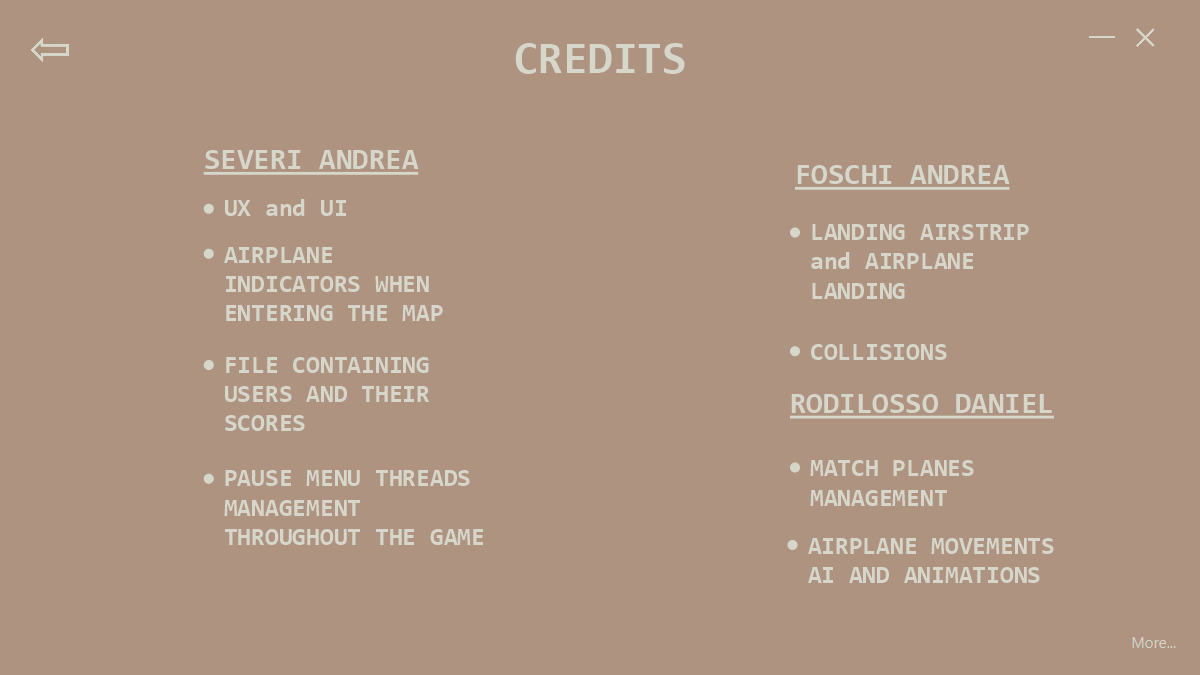
\includegraphics[width=\textwidth]{img/GuidaUtente/Credits.png}
    \end{center}
    \caption{Riconoscimenti}
    \label{img:credits}
\end{figure}

\clearpage

\section*{Partita}
All'avvio della partita, la mappa Seaside si presenterà così con l'opzione di poter mettere in pausa il gioco e uscire o riprendere successivamente.
\begin{figure}[H]
    \begin{center}
        \centering
        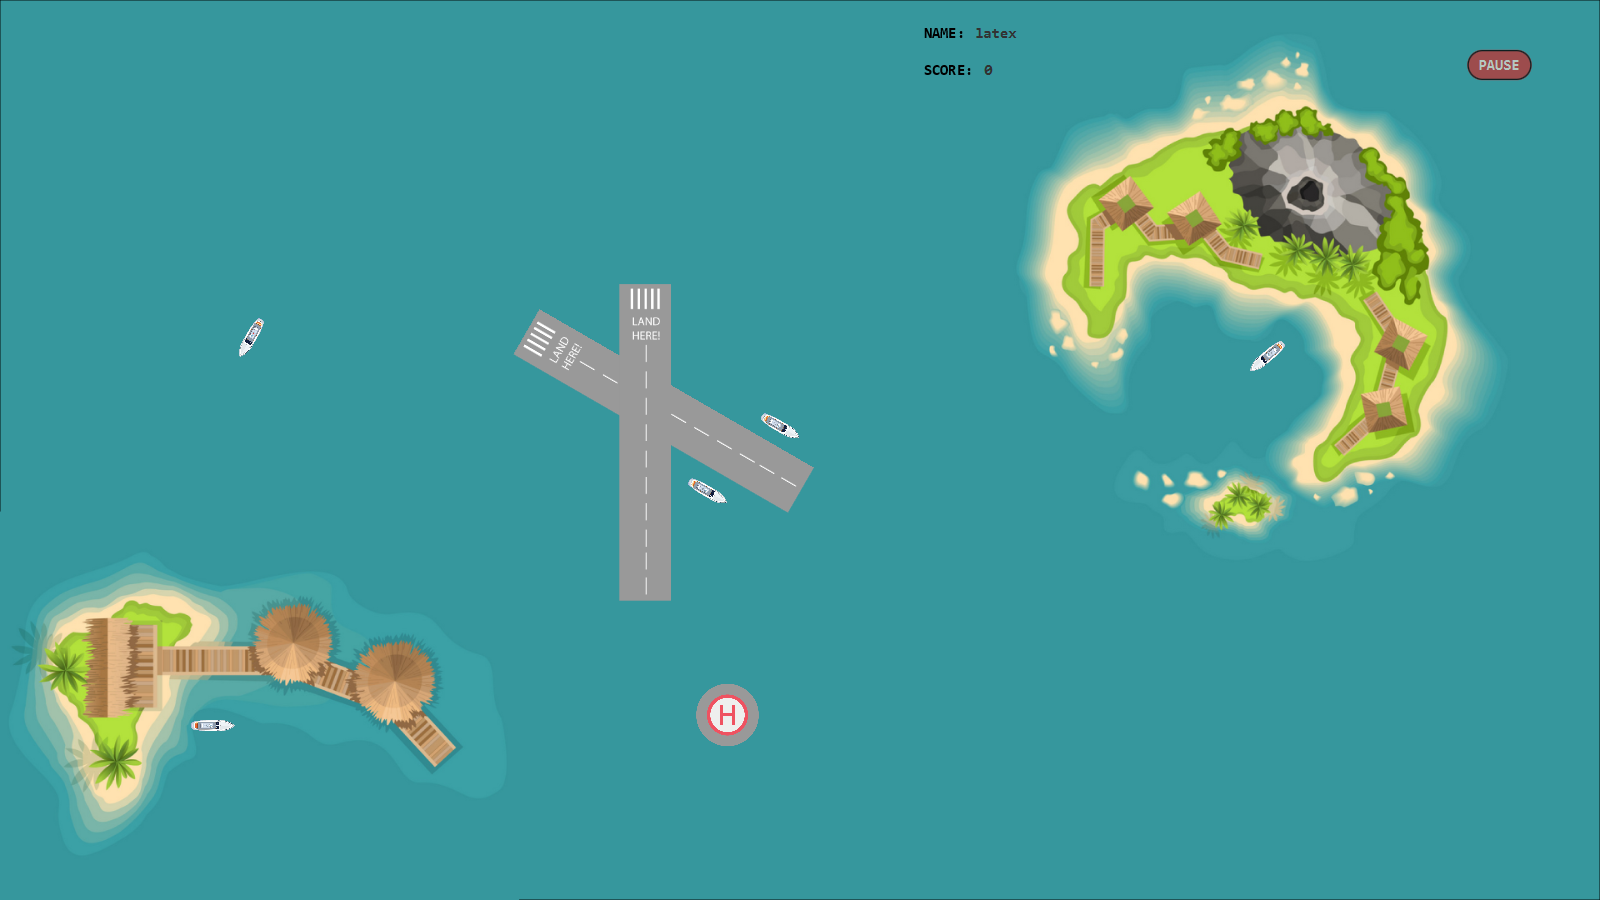
\includegraphics[width=\textwidth]{img/GuidaUtente/Seaside.png}
    \end{center}
    \caption{Mappa di gioco}
    \label{img:seaside}
\end{figure}
\end{document}
